\documentclass[11pt,a4paper]{article}

\usepackage[T1]{fontenc}
\usepackage[utf8]{inputenc}
\usepackage{lmodern}
\usepackage[margin=2.6cm]{geometry}
\usepackage{amsmath,amssymb}
\usepackage{booktabs}
\usepackage{tabularx}
\usepackage{array}
\usepackage{tikz}
\usepackage{caption}
\usepackage{microtype}
\usepackage[round,sort]{natbib}
\usepackage[hidelinks]{hyperref}

\captionsetup{font=small,labelfont=bf}

\title{Forecasting Fantasy Premier League Points:\\
A Walk-Forward Evaluation of Captaincy and Lineup Decisions}
\author{[Author name]\\[2pt]\small [Affiliation]}
\date{October 2026}

\begin{document}
\maketitle

\begin{abstract}
\noindent
Fantasy Premier League (FPL) managers choose, every week, eleven starters from a fifteen-player
squad and a captain whose points are doubled. We forecast each player's points for the coming
gameweek with gradient-boosted regression trees trained on four seasons of player-level match
data (2022/23--2025/26; 79{,}885 player-gameweeks), using only information available before
each deadline. The model is evaluated walk-forward over 114 gameweeks (2023/24--2025/26),
retrained every week on all earlier weeks, and its decisions are compared with fixed baselines
under an acceptance rule stated before the first run. The forecast is more accurate than recent
form (mean absolute error 1.42 versus 1.50 points; correlation 0.51 versus 0.41). As a captain
rule it outscores choosing the most expensive attacker who started the previous week by $+1.54$
points per week (95\% bootstrap interval $+0.45$ to $+2.61$) and choosing the best recent form by
$+1.44$ ($+0.27$ to $+2.62$), but trails the captain most often chosen by the managers who
finished the season in the overall top 100 by $-1.46$ ($-2.40$ to $-0.55$). Selecting starting
elevens from those managers' actual squads, the model beats a form rule by $+2.39$ points per week
but trails the managers' own choices by $-2.16$. Ablations show which inputs carry the forecast,
and the conclusions are stable across model settings. We also test whether a player's share of
his team's possession-ending actions, an adaptation of basketball's usage rate, adds information.
We discuss why the strongest baseline is both informative and biased, and why single-season
evaluations cannot separate decision rules that differ by less than about one point per week.
\end{abstract}

\section{Introduction}

Fantasy Premier League is the official fantasy game of the English Premier League. Each manager
holds fifteen players within a fixed budget and, before each of the season's 38 gameweek
deadlines, names eleven starters and a captain whose points are doubled \citep{fplrules}. Players
score for playing time, goals, assists, clean sheets, saves and bonus points and, from 2025/26,
for defensive actions. Two decisions recur every week regardless of transfers: who starts, and
who captains. Both reduce to ranking players by expected points in the coming week.

A small literature forecasts FPL points with statistical and machine-learning models. Early
work treated team selection as sequential decision-making under uncertainty
\citep{matthews2012}. Later studies forecast points from recent match histories using time-series
and recurrent models \citep{gupta2019}, convolutional and recurrent networks over a player's last
five matches \citep{lombu2024}, and ridge regression, gradient boosting and convolutional networks
\citep{frees2024}. Others add information beyond match statistics, such as news and betting
markets \citep{bonello2019}, or couple forecasts with mixed-integer squad selection
\citep{ramezani2025}. These studies mostly report forecast error or season-long team totals.
Fewer ask whether forecasts make better \emph{weekly decisions} than the rules and expert
consensus managers already use, and fewer fix the criterion for success before looking at the
results.

This paper asks that question. We are explicit about two things that often go unstated in
sports forecasting: information leakage, meaning the use of data that would not have been known
at decision time \citep{tashman2000}, and the noise of weekly outcomes, which limits what any
evaluation can show. Our contributions are:
\begin{enumerate}
  \item a deadline-safe feature set that carries players' form across seasons and uses the
        previous season's rates as a prior, following the logic of empirical Bayes shrinkage
        \citep{efronmorris1975,brown2008};
  \item a walk-forward evaluation that retrains every week and compares \emph{decisions}
        against fixed baselines, with an acceptance rule set in advance \citep{nosek2018};
  \item lineup evaluation on 11{,}400 real squads, with substitutions applied by the game's
        rules;
  \item ablation and sensitivity analyses, so that results do not rest on unexamined
        choices; and
  \item a test of whether ball usage, adapted from basketball's usage rate
        \citep{bbrefglossary,oliver2004}, adds information.
\end{enumerate}

\section{Data}

\subsection{Player-gameweek records}
We use official FPL data for four complete seasons, 2022/23 to 2025/26
\citep{fplapi}. Fixture lists and club identifiers for past seasons come from a public archive of
the same data \citep{anandfpl}. For every player and gameweek we record:
\begin{itemize}
  \item minutes, starts, goals, assists, clean sheets, goals conceded and saves;
  \item bonus points and the bonus points system score;
  \item expected goals (xG), expected assists (xA) and expected goals conceded;
  \item total FPL points.
\end{itemize}
Expected goals estimate the probability that a shot is scored from its location and context
\citep{rathke2017}; FPL publishes Opta's values. In a double gameweek, when a club plays twice,
the two matches are summed. Players and clubs keep the same identifier across seasons. Players
with no minutes in a season are excluded for that season (Table~\ref{tab:data}). Because fixtures
are known, a week with no fixture (a blank gameweek) is distinguished from a week in which a
player did not play.

\begin{table}[ht]
\centering
\caption{Player-gameweek records by season.}
\label{tab:data}
\begin{tabular}{lrrr}
\toprule
Season & Player-gameweeks & Players & Total FPL points \\
\midrule
2022/23 & 19{,}501 & 554 & 31{,}724 \\
2023/24 & 20{,}526 & 570 & 31{,}273 \\
2024/25 & 20{,}215 & 562 & 31{,}291 \\
2025/26 & 19{,}643 & 537 & 34{,}382 \\
\midrule
Total   & 79{,}885 &     &           \\
\bottomrule
\end{tabular}
\end{table}

Weekly prices were not archived, so each player carries his start-of-season price. The 2025/26
scoring rules added points for defensive actions \citep{fplrules}, which partly explains that
season's higher total.

\subsection{Squads of top-ranked managers}
For 2023/24 to 2025/26 we hold the weekly fifteen-player squads, starting elevens, bench order,
captain and vice-captain of the 100 managers who finished each season in the overall top 100:
$3\times38\times100 = 11{,}400$ squad-weeks. Their most-captained player is a baseline, and their
squads are a realistic test bed for lineup decisions. The sample is selected on the outcome: these
managers are included \emph{because} their season went well. Selecting on survival inflates
apparent performance, a problem documented for investment funds \citep{brown1992}, and it
matters here (Section~\ref{sec:discussion}).

\subsection{Season event data}
For the usage analysis (Section~\ref{sec:usage}) we use Opta season totals for every Premier
League player from 2021/22 to 2025/26, published through the Premier League's statistics
services \citep{plstats}. Each player is assigned to the club he played for that season, taken
from the season's squad lists, or, for players who left mid-season, from the club where he
played most of his minutes.

\section{Method}

\subsection{Notation and the information constraint}
Index players by $i$, seasons by $s$ and gameweeks by $g$, and write $t=(s,g)$ for a point in time
ordered lexicographically. Let $y_{it}$ be player $i$'s points in week $t$, $m_{it}$ his minutes and
$n_{it}\in\{0,1,2\}$ the number of fixtures his club plays. The forecast for week $t$ may use only
weeks $t'<t$, together with quantities fixed before the deadline (position, start-of-season price,
the fixture list, and the previous season's totals). We test this by perturbing the outcomes of one
week and confirming that features for that week and all earlier weeks are unchanged.

\subsection{Features}
Player state is updated after each week in which the player's club had a fixture; the features
for week $t$ take the most recent state from a strictly earlier week. Table~\ref{tab:choices}
lists each design choice with its basis.

\paragraph{Form and role.} Minutes per fixture in the last week and averaged over the last three
and six club-fixture weeks; the share of fixtures started over the last six; points per fixture
over the last three and six. Short rolling windows of recent matches are the common input in FPL
forecasting \citep{lombu2024,frees2024,ramezani2025}.

\paragraph{Per-90 rates.} Over the last six club-fixture weeks $\mathcal{W}_6$, for a statistic
$z$ (xG, xA, bonus, bonus points system score, saves),
\[
  r^{(6)}_{it}(z) = 90 \cdot \frac{\sum_{t'\in\mathcal{W}_6} z_{it'}}{\max\!\bigl(\sum_{t'\in\mathcal{W}_6} m_{it'},\,90\bigr)},
\]
where the floor of 90 minutes stops a short cameo from producing an extreme rate.

\paragraph{Season to date.} The same rates for xG, xA and points accumulated over the current
season; the share of available minutes played, $\sum m / (90\sum n)$; and the number of fixtures
so far. These are missing in a season's first week.

\paragraph{Prior season.} The player's xG, xA and points per 90, and his share of the season's
minutes, in the previous season. Early in a season the current sample is a few matches and
observed rates are dominated by noise. Combining them with a longer-run prior is the principle
behind empirical Bayes estimation, which in sport outperforms the raw early-season rate
\citep{efronmorris1975,brown2008}. Here the trees learn how much weight the prior deserves at each
point of the season; Section~\ref{sec:sensitivity} tests whether it helps.

\paragraph{Club and opponent strength.} For club $c$ in week $t$, let
$G^{+}_{ct}=\sum_{i\in c}\mathrm{xG}_{it}$ be its xG and
$G^{-}_{ct}=\sum_{o} G^{+}_{ot}/n_{ot}$ its xG conceded, summing over its opponents $o$ that week.
Over the previous eight gameweeks, the club's attacking and defensive strength are
\[
  A_{ct} = \frac{\sum_{t'} G^{+}_{ct'}}{\sum_{t'} n_{ct'}}, \qquad
  D_{ct} = \frac{\sum_{t'} G^{-}_{ct'}}{\sum_{t'} n_{ct'}}.
\]
Separate attack and defence parameters per club are the basis of the standard goal models for
football \citep{maher1982,dixoncoles1997}. We estimate them from xG rather than goals because xG
is less noisy over short windows \citep{rathke2017}. The player receives his club's $A$ and $D$,
the average of his opponents' $A$ and $D$ in week $t$, the number of fixtures, and the share
played at home.

\paragraph{Static.} Position, start-of-season price, gameweek number, an indicator for the
defensive-action scoring rules, appearances to date, and the number of weeks since his last
club-fixture week.

\begin{table}[ht]
\centering
\small
\caption{Design choices and their basis.}
\label{tab:choices}
\begin{tabularx}{\textwidth}{>{\raggedright\arraybackslash}p{4.2cm}X}
\toprule
Choice & Basis \\
\midrule
Previous-season rates as a prior & Shrinkage of noisy early-season rates
  \citep{efronmorris1975,brown2008}; no average gain in ablation (Table~\ref{tab:sensitivity}) \\
Rolling windows of recent matches & Standard in FPL forecasting
  \citep{lombu2024,frees2024,ramezani2025} \\
Club attack/defence strength & Goal models with team attack and defence parameters
  \citep{maher1982,dixoncoles1997}; xG as a lower-noise input \citep{rathke2017} \\
Gradient-boosted trees & \citet{friedman2001}; histogram variant \citep{ke2017}; used for FPL
  by \citet{frees2024} \\
Model settings & Fixed before evaluation; sensitivity reported in Table~\ref{tab:sensitivity} \\
Walk-forward evaluation & Rolling-origin out-of-sample testing
  \citep{tashman2000,bergmeir2012} \\
Paired comparison by week & Comparing forecasts on common outcomes \citep{dieboldmariano1995};
  weeks resampled by bootstrap \citep{efron1993} \\
Acceptance rule set in advance & Pre-registration \citep{nosek2018} \\
Usage rate & Basketball usage percentage \citep{bbrefglossary,oliver2004}; football adaptation
  \citep{sincerefc2025a,sincerefc2025b} \\
\bottomrule
\end{tabularx}
\end{table}

\subsection{Model}
The target is $y_{it}$, the player's total points in week $t$. We fit a gradient-boosted
ensemble of regression trees \citep{friedman2001} with histogram binning of the inputs
\citep{ke2017}, as implemented in scikit-learn \citep{pedregosa2011}, minimising squared error.
The settings are:
\begin{itemize}
  \item learning rate 0.05 and at most 250 boosting iterations, stopped early when the loss on a
        random 10\% of the training window stops improving for ten iterations (the library's
        default whenever there are more than 10{,}000 training rows);
  \item at most 31 leaves per tree;
  \item at least 80 observations per leaf;
  \item an $L_2$ penalty of 1.0.
\end{itemize}
They start from the library defaults (learning rate 0.1, 100 iterations, 20 observations per
leaf, no penalty) and move each setting in the conservative direction suited to a noisy target.
They were fixed before evaluation and not tuned on the test seasons; Section~\ref{sec:sensitivity}
reports the effect of changing them.

Missing inputs, such as prior-season rates for a player new to the league, are handled natively
by the trees. Features that are constant or entirely missing within a training window are dropped
for that fit. A player with no previous club-fixture weeks receives no forecast. Training uses
every player-week with a fixture and at least one prior observation. Squared error makes the
forecast an estimate of the conditional mean, the right target for a captain choice that
maximises expected points.

\subsection{Decision rules}
\paragraph{Captain.} In each test week, the model captains the player with the highest
forecast among those whose club has a fixture.

\paragraph{Lineup.} Given a fifteen-player squad, the model chooses the legal formation that
maximises the sum of forecasts. A formation has one goalkeeper, $d$ defenders, $m$ midfielders
and $f$ forwards, with $d\in\{3,4,5\}$, $m\in\{2,\dots,5\}$, $f\in\{1,2,3\}$ and $d+m+f=10$. The
two highest forecasts in the eleven are captain and vice-captain. The bench lists the reserve
goalkeeper first and the outfield players by forecast.

\paragraph{Scoring.} Every strategy is scored by the game's ordinary rules \citep{fplrules}. A
starter with no minutes is replaced by the first bench player, in bench order, who played and
whose entry keeps the formation legal (goalkeeper for goalkeeper; at least three defenders, two
midfielders and one forward). The captain's points are doubled; if he did not play, the
vice-captain's are. Chips are ignored: a triple captain counts as an ordinary captain and a
bench boost as an ordinary week.

\subsection{Baselines}
All baselines use only information available at the deadline.
\begin{description}
  \item[Top-100 consensus.] The player most often captained that week by the 100 managers who
        finished the season in the overall top 100. This is the collective judgement of strong
        managers \citep{surowiecki2004}, but the group is defined after the fact.
  \item[Premium attacker.] The most expensive midfielder or forward (by start-of-season price)
        who played at least 60 minutes per fixture in his previous club-fixture week. Ties are
        broken by points per fixture over the last six.
  \item[Recent form.] The highest points per fixture over the last six, among players averaging
        at least 60 minutes per fixture over the last three.
\end{description}
For lineups, the baselines are the manager's actual eleven, bench order and captain, and the
model's own selection procedure ranking players by recent form.

\subsection{Evaluation}
For each test week $w$ the model is retrained on all weeks before $w$, including earlier weeks of
the same season, and used to forecast week $w$. This rolling-origin design mirrors live use
\citep{tashman2000} and avoids the leakage that random cross-validation introduces in time-ordered
data \citep{bergmeir2012}. The test period is the 114 gameweeks of 2023/24, 2024/25 and 2025/26.

Comparisons are paired by week, so that two rules are judged on the same outcomes
\citep{dieboldmariano1995}. For rule $A$ and baseline $B$, let
$d_w=\mathrm{pts}_w(A)-\mathrm{pts}_w(B)$; for lineups, $\mathrm{pts}_w$ is first averaged over the 100
squads in week $w$. Weeks are the unit of resampling, since players and squads within a week share
the same matches. We report $\bar d$ with a 95\% percentile interval from 10{,}000 bootstrap
resamples of the 114 weekly differences \citep{efron1993}.

\paragraph{Acceptance rule.} Stated before the first evaluation: the model's captain choice is
accepted only if the lower end of the interval is above zero against \emph{every} captain
baseline. The same rule applies to lineups. The absence of a detectable difference is not treated
as evidence of parity.

\paragraph{Forecast accuracy.} We report the mean absolute error (MAE) and the Pearson correlation
of forecasts with outcomes over all test player-weeks with a fixture. We compare against a form
forecast: points per fixture over the last six or, where unavailable, the prior season's points
per 90 scaled by the player's share of minutes.

\section{Results}

\subsection{Forecast accuracy}
Over 58{,}682 test player-weeks, the model's MAE is 1.42 points against 1.50 for recent form, and
its correlation with outcomes is 0.51 against 0.41 (Table~\ref{tab:accuracy}). Most player-weeks
score two points or fewer, so the correlation is the more informative comparison of ranking
ability.

\begin{table}[ht]
\centering
\caption{Forecast accuracy over all test player-weeks with a fixture (2023/24--2025/26).}
\label{tab:accuracy}
\begin{tabular}{lcc}
\toprule
 & Mean absolute error (points) & Correlation with outcome \\
\midrule
Model       & 1.42 & 0.51 \\
Recent form & 1.50 & 0.41 \\
\bottomrule
\end{tabular}
\end{table}

\subsection{Captaincy}
Table~\ref{tab:captain} gives each rule's captain points per week (single, not doubled), and
Figure~\ref{fig:intervals} the paired differences.
\begin{itemize}
  \item The model averages 6.75 points per week.
  \item It outscores the premium-attacker rule by $+1.54$ (95\% interval $+0.45$ to $+2.61$) and
        the recent-form rule by $+1.44$ ($+0.27$ to $+2.62$).
  \item It trails the top-100 consensus captain by $-1.46$ ($-2.40$ to $-0.55$), so under the
        stated rule it is \emph{not accepted}.
  \item The best possible captain each week scored 17.79 points on average, a mean regret of
        11.04 points.
\end{itemize}
In 2023/24 the premium-attacker rule outscored the model (6.05 against 5.21); only in the two
later seasons does the model clearly lead the mechanical rules. The top-100 consensus leads in
every season.

\begin{table}[ht]
\centering
\caption{Captain points per gameweek (single) by season.}
\label{tab:captain}
\begin{tabular}{lcccc}
\toprule
Season & Model & Top-100 consensus & Premium attacker & Recent form \\
\midrule
2023/24 & 5.21 & 7.29 & 6.05 & 4.87 \\
2024/25 & 8.82 & 10.13 & 5.26 & 6.71 \\
2025/26 & 6.21 & 7.18 & 4.29 & 4.34 \\
\midrule
All (114 weeks) & 6.75 & 8.20 & 5.20 & 5.31 \\
\bottomrule
\end{tabular}
\end{table}

\begin{figure}[ht]
\centering
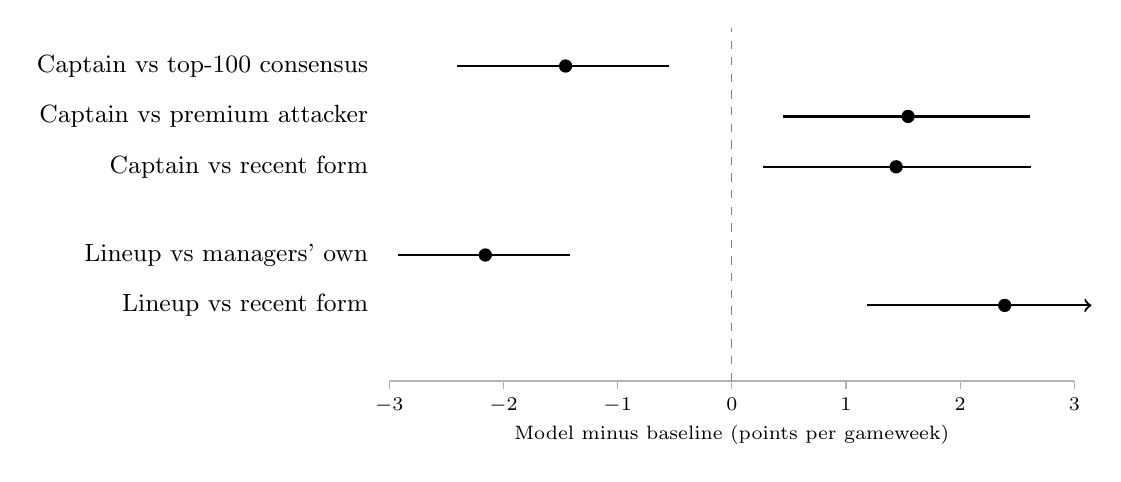
\begin{tikzpicture}[x=1.45cm,y=0.8cm]
  \draw[gray!60] (-3,0.4) -- (3,0.4);
  \foreach \x in {-3,-2,-1,0,1,2,3} {
    \draw[gray!60] (\x,0.4) -- (\x,0.28) node[below,font=\scriptsize,text=black] {$\x$};
  }
  \draw[dashed,gray] (0,0.4) -- (0,6.0);
  \node[font=\scriptsize] at (0,-0.45) {Model minus baseline (points per gameweek)};
  \node[anchor=east,font=\small] at (-3.1,5.4) {Captain vs top-100 consensus};
  \draw[thick] (-2.404,5.4) -- (-0.553,5.4); \fill (-1.456,5.4) circle (2.4pt);
  \node[anchor=east,font=\small] at (-3.1,4.6) {Captain vs premium attacker};
  \draw[thick] (0.447,4.6) -- (2.614,4.6); \fill (1.544,4.6) circle (2.4pt);
  \node[anchor=east,font=\small] at (-3.1,3.8) {Captain vs recent form};
  \draw[thick] (0.272,3.8) -- (2.623,3.8); \fill (1.439,3.8) circle (2.4pt);
  \node[anchor=east,font=\small] at (-3.1,2.4) {Lineup vs managers' own};
  \draw[thick] (-2.923,2.4) -- (-1.421,2.4); \fill (-2.159,2.4) circle (2.4pt);
  \node[anchor=east,font=\small] at (-3.1,1.6) {Lineup vs recent form};
  \draw[thick] (1.185,1.6) -- (3.0,1.6); \draw[thick,->] (2.9,1.6) -- (3.15,1.6);
  \fill (2.39,1.6) circle (2.4pt);
\end{tikzpicture}
\caption{Paired weekly differences with 95\% bootstrap intervals over 114 gameweeks. Points to the
right of zero favour the model. The upper end of the last interval ($+3.61$) lies beyond the axis.}
\label{fig:intervals}
\end{figure}

\subsection{Lineups}
On the 11{,}400 top-100 squad-weeks, the model's elevens and captains score 66.13 points per
squad-week, against 68.29 for the managers' own choices and 63.74 for the form rule. The model
beats the form rule by $+2.39$ ($+1.19$ to $+3.61$) and trails the managers by $-2.16$
($-2.92$ to $-1.42$); it is not accepted for lineups either.

\subsection{Which inputs matter, and how fragile are the settings?}\label{sec:sensitivity}
Table~\ref{tab:sensitivity} repeats the full walk-forward evaluation with one change at a time:
a block of features removed, or one model setting moved. All runs, including the headline results,
use the same software environment (scikit-learn 1.9.1, pandas 3.0.6, NumPy 2.4.6).
\IfFileExists{sensitivity_table.tex}{%
\begin{table}[ht]
\centering
\small
\caption{Ablations and sensitivity. MAE and correlation over all test player-weeks; captain
points per week; and the captain's mean weekly difference from the top-100 consensus and premium
baselines. Each row is a full walk-forward run over 2023/24--2025/26.}
\label{tab:sensitivity}
\begin{tabular}{lcccccc}
\toprule
 & MAE & Corr. & Captain & vs top-100 & vs premium & vs form, lower CI \\
\midrule
Reference model & 0.996 & 0.575 & 6.61 & $-1.59$ & $+1.46$ & $+0.22$ \\
\midrule
Without prior season & 0.996 & 0.576 & 6.89 & $-1.32$ & $+1.73$ & $+0.44$ \\
Without club and opponent strength & 1.005 & 0.571 & 6.91 & $-1.29$ & $+1.75$ & $+0.52$ \\
Without per-90 rates (last six) & 0.996 & 0.574 & 6.51 & $-1.69$ & $+1.35$ & $+0.13$ \\
Without season to date & 1.004 & 0.572 & 6.79 & $-1.41$ & $+1.63$ & $+0.33$ \\
Without minutes and starts & 1.014 & 0.560 & 6.33 & $-1.88$ & $+1.17$ & $-0.10$ \\
\midrule
Learning rate 0.1, 125 iterations & 0.995 & 0.574 & 6.71 & $-1.49$ & $+1.55$ & $+0.18$ \\
15 leaves per tree & 0.993 & 0.577 & 6.76 & $-1.44$ & $+1.60$ & $+0.35$ \\
63 leaves per tree & 0.997 & 0.574 & 7.14 & $-1.06$ & $+1.98$ & $+0.82$ \\
20 observations per leaf & 0.995 & 0.575 & 6.96 & $-1.24$ & $+1.81$ & $+0.72$ \\
Library defaults & 0.998 & 0.572 & 6.99 & $-1.21$ & $+1.83$ & $+0.69$ \\
\bottomrule
\end{tabular}

\end{table}}{\textit{[Sensitivity table pending.]}}

Three findings stand out.
\begin{itemize}
  \item \emph{Accuracy depends most on minutes and starts.} Removing them raises MAE from 1.415
        to 1.442 and lowers correlation from 0.508 to 0.488, the largest loss of any block. Club
        and opponent strength (1.427, 0.501) and season-to-date rates (1.424, 0.502) come next.
  \item \emph{Last season's rates add nothing on average.} Removing them leaves MAE and
        correlation unchanged (1.415, 0.508). The motivation for including them, stabilising
        early-season estimates, is not borne out over whole seasons. Carrying the rolling
        windows across season boundaries and the start-of-season price may already supply that
        information. Whether the prior helps in the first weeks alone is not tested here.
  \item \emph{The conclusions do not depend on the settings.} Across all eleven variants, MAE
        stays within 0.027 and correlation within 0.020 of the reference. Captain points range
        from 6.25 to 7.10 per week, but every variant still beats the premium-attacker rule
        (lower interval bounds $+0.02$ or above) and still trails the top-100 consensus (upper
        bounds $-0.22$ or below). The acceptance verdict is the same in every row.
\end{itemize}
The spread in captain points is itself informative. A preliminary run of the same variants under
an earlier library version moved several of them in the opposite direction (for example, 63
leaves per tree gave 6.50 there and 7.10 here). Differences of half a point per week in captain
points are within the noise of three seasons (Section~\ref{sec:discussion}). They should not be
used to choose settings, and we have not done so.

\section{Extension: ball usage}\label{sec:usage}

\subsection{Motivation and definition}
In basketball, usage percentage estimates the share of a team's possessions a player ends with a
shot, free throws or a turnover while he is on the floor \citep{bbrefglossary}. It builds on the
possession-based framework of \citet{oliver2004}. It separates how much of the ball a player
consumes from what he produces with it. A recent football adaptation
\citep{sincerefc2025a,sincerefc2025b} counts \emph{possession-ending actions}: shots, and every way
of losing the ball (an incomplete pass or cross, a failed take-on, being tackled or dispossessed,
a miscontrol). It argues that the measure describes a player's role and hierarchy within a team.
A player used to being his team's main option may struggle to produce when he joins a club that
already has one. If so, last season's usage should carry information about this season's output,
especially for players who change club, where the prior-season rates in our model are least
reliable.

We define a player's possession-ending actions as Opta's possessions lost plus his shots.
Possessions lost covers incomplete passes and crosses, failed take-ons, being tackled and
miscontrols, and a little more: for Premier League players with at least 1{,}500 minutes in
2023/24--2025/26 it is a median 8\% larger than the sum of those itemised components (middle 90\%
of players: 1\% to 32\% larger). Following the basketball formula with eleven players in
place of five,
\[
  \mathrm{USG}_i = 100\cdot\frac{\mathrm{PEA}_i\cdot(\text{team minutes}/11)}{\text{minutes}_i\cdot\mathrm{PEA}_{\text{team}}},
\]
where team totals are taken over every player of the club he played for that season. For
creation we use Opta's chances created: passes that lead directly to a shot. The adaptation
above uses a broader measure of shot-creating actions, which our source does not publish.

\subsection{Features and test}
We add eight features computed from the \emph{previous} season's totals, so all are known
before the season being forecast:
\begin{itemize}
  \item usage rate;
  \item possession-ending actions per 90;
  \item chances created per 90;
  \item chances created per possession-ending action;
  \item touches in the opposition box per 90;
  \item the club's possession share;
  \item an indicator that the player has changed club;
  \item the highest previous-season usage among his current teammates.
\end{itemize}
The last feature asks whether the club he now plays for already has a dominant ball user. We
then rerun the walk-forward evaluation with and without these features on identical weeks, and
bootstrap the paired weekly differences.

\IfFileExists{usage_table.tex}{%
\begin{table}[ht]
\centering
\small
\caption{Walk-forward evaluation with and without the usage features (2023/24--2025/26).
Differences are with-usage minus without, paired by gameweek, with 95\% bootstrap intervals.
$^a$Reduction in MAE (positive means the usage features help).}
\label{tab:usage}
\begin{tabular}{lccc}
\toprule
 & Without usage & With usage & Difference (95\% CI) \\
\midrule
Mean absolute error$^a$ & 0.996 & 0.993 & $+0.003$ ($+0.001$ to $+0.004$) \\
Correlation & 0.575 & 0.576 & \\
Captain points per week & 6.61 & 6.92 & $+0.31$ ($-0.24$ to $+0.85$) \\
Lineup points per week & 66.00 & 66.05 & $+0.04$ ($-0.35$ to $+0.43$) \\
MAE, players who changed club$^a$ & & & $+0.002$ ($-0.003$ to $+0.007$) \\
\bottomrule
\end{tabular}

\end{table}}{\textit{[Usage results pending.]}}

\subsection{Result}
The usage features were present for 57\% of test player-weeks; the rest belong to players with
no Premier League season the year before. Players who had changed club since the previous season
account for 10\% of test player-weeks. Table~\ref{tab:usage} shows no detectable effect:
\begin{itemize}
  \item forecast error is unchanged (MAE reduction $0.000$, 95\% interval $-0.003$ to $+0.003$),
        including for players who changed club ($+0.001$, $-0.005$ to $+0.006$);
  \item captain points change by $-0.27$ per week ($-1.26$ to $+0.69$);
  \item lineup points are unchanged ($+0.00$, $-0.71$ to $+0.74$).
\end{itemize}
Over these three seasons, last season's ball usage adds nothing that last season's xG, xA, points
and minutes do not already carry, so we do not adopt it. Two caveats apply. First, the measure is
a season total; an in-season, match-level version would capture role changes as they happen.
Second, usage may matter for questions this model does not ask, such as how a new signing's
arrival redistributes the ball among his teammates, which needs club-level rather than
player-level modelling.

\section{Discussion}\label{sec:discussion}

\paragraph{What the model has learned.} The forecast ranks players better than recent points do:
its correlation with outcomes is about a quarter higher. As a decision rule it beats both
mechanical captain heuristics, and it picks better elevens than form does from the same squads.
These gains come mainly from minutes security, club and opponent strength and current-season
rates (Section~\ref{sec:sensitivity}), and from not over-reacting to a short run of high or low
scores. Neither last season's rates nor last season's ball usage improved the forecast on
average.

\paragraph{Why the top-100 consensus is hard to beat.} The consensus baseline has two advantages.
The first is genuine. At the deadline, managers know team news, late injuries, the likely penalty
taker and the betting market's view of each fixture, none of which the model sees. Betting
markets in particular are known to carry information beyond statistical models
\citep{dixoncoles1997}, and adding news and market data has improved FPL forecasts in earlier work
\citep{bonello2019}. The second is an artefact of selection. These managers are in the sample
because their season went well, so their captaincy choices are, on average, those that worked out
\citep{brown1992}. A fair comparison would use the consensus of a sample fixed before the season.

\paragraph{How much evidence a season provides.} Inverting the reported intervals gives a
standard deviation of the weekly paired captain difference of roughly 5 to 6 points: for the
top-100 comparison, $\hat\sigma\approx0.93\sqrt{114}/1.96\approx5.0$. With $\sigma=5$, a 95\%
interval of half-width $h$ requires about $(1.96\,\sigma/h)^2$ weeks. That is 96 weeks for $h=1$
point and about 380 weeks for $h=0.5$; a single season gives $h\approx1.6$. Claims that one
captaincy rule beats another by half a point per week cannot be supported by one season, or even
three.

\paragraph{Limitations.}
\begin{itemize}
  \item \emph{Missing information.} The model has no team news, injury history, set-piece
        duties or bookmaker prices.
  \item \emph{Prices.} Only start-of-season prices are available historically.
  \item \emph{Selection on the outcome.} The top-100 sample is selected on how the season
        turned out.
  \item \emph{Serial dependence.} Weekly differences may be serially dependent within a season;
        a block or stationary bootstrap \citep{kunsch1989,politis1994} would widen the intervals
        somewhat.
  \item \emph{Reuse of the test seasons.} The usage extension and any further development
        evaluated on these same three seasons risk overstating performance; improvements should
        be confirmed prospectively.
\end{itemize}

\paragraph{Prospective evaluation.} From the seventh gameweek of 2026/27, the following
captains are logged before each deadline:
\begin{itemize}
  \item the model's;
  \item the one implied by the official game's expected-points figure;
  \item the premium-attacker rule's.
\end{itemize}
The most-captained player across all managers is recorded once the gameweek begins. Logs are
frozen at the deadline and scored when the gameweek finishes. The official expected points,
ownership and availability flags are stored at each deadline. This closes part of the
information gap for future model versions and gives an out-of-sample record that cannot be
revised with hindsight.

\section{Conclusion}
A gradient-boosted forecast trained on four seasons of public data makes better captain and
lineup choices than simple rules, and ranks players better than recent form. It does not yet
match the collective judgement of the season's best managers, whose advantage reflects both
information the model lacks and the way they were selected. Distinguishing good rules from
slightly better ones requires many more weeks than a season provides. Evaluation should therefore
be prospective, pre-specified and patient.

\begin{thebibliography}{30}
\setlength{\itemsep}{2pt}\small

\bibitem[Anand(2026)]{anandfpl}
V.~Anand.
\newblock Fantasy-Premier-League: a library and dataset of historical FPL data.
\newblock GitHub repository, \url{https://github.com/vaastav/Fantasy-Premier-League}, accessed October 2026.

\bibitem[Basketball-Reference(2026)]{bbrefglossary}
Basketball-Reference.
\newblock Glossary: usage percentage.
\newblock \url{https://www.basketball-reference.com/about/glossary.html}, accessed October 2026.

\bibitem[Bergmeir and Ben\'itez(2012)]{bergmeir2012}
C.~Bergmeir and J.~M. Ben\'itez.
\newblock On the use of cross-validation for time series predictor evaluation.
\newblock \emph{Information Sciences}, 191:192--213, 2012.

\bibitem[Bonello et~al.(2019)]{bonello2019}
N.~Bonello, J.~Beel, S.~Lawless, and J.~Debattista.
\newblock Multi-stream data analytics for enhanced performance prediction in fantasy football.
\newblock In \emph{Proceedings of the 27th Irish Conference on Artificial Intelligence and Cognitive Science (AICS)}, pages 284--292, 2019.

\bibitem[Brown(2008)]{brown2008}
L.~D. Brown.
\newblock In-season prediction of batting averages: a field test of empirical Bayes and Bayes methodologies.
\newblock \emph{Annals of Applied Statistics}, 2(1):113--152, 2008.

\bibitem[Brown et~al.(1992)]{brown1992}
S.~J. Brown, W.~Goetzmann, R.~G. Ibbotson, and S.~A. Ross.
\newblock Survivorship bias in performance studies.
\newblock \emph{Review of Financial Studies}, 5(4):553--580, 1992.

\bibitem[Diebold and Mariano(1995)]{dieboldmariano1995}
F.~X. Diebold and R.~S. Mariano.
\newblock Comparing predictive accuracy.
\newblock \emph{Journal of Business \& Economic Statistics}, 13(3):253--263, 1995.

\bibitem[Dixon and Coles(1997)]{dixoncoles1997}
M.~J. Dixon and S.~G. Coles.
\newblock Modelling association football scores and inefficiencies in the football betting market.
\newblock \emph{Journal of the Royal Statistical Society: Series C}, 46(2):265--280, 1997.

\bibitem[Efron and Morris(1975)]{efronmorris1975}
B.~Efron and C.~Morris.
\newblock Data analysis using Stein's estimator and its generalizations.
\newblock \emph{Journal of the American Statistical Association}, 70(350):311--319, 1975.

\bibitem[Efron and Tibshirani(1993)]{efron1993}
B.~Efron and R.~J. Tibshirani.
\newblock \emph{An Introduction to the Bootstrap}.
\newblock Chapman \& Hall, 1993.

\bibitem[Fantasy Premier League(2026a)]{fplapi}
Fantasy Premier League.
\newblock Public data endpoints (bootstrap, fixtures, element summaries, live gameweek data).
\newblock \url{https://fantasy.premierleague.com/api/}, accessed 2022--2026.

\bibitem[Fantasy Premier League(2026b)]{fplrules}
Fantasy Premier League.
\newblock Rules.
\newblock \url{https://fantasy.premierleague.com/help/rules}, accessed October 2026.

\bibitem[Frees et~al.(2024)]{frees2024}
D.~Frees, P.~Ravella, and C.~Zhang.
\newblock Deep learning and transfer learning architectures for English Premier League player performance forecasting.
\newblock arXiv:2405.02412, 2024.

\bibitem[Friedman(2001)]{friedman2001}
J.~H. Friedman.
\newblock Greedy function approximation: a gradient boosting machine.
\newblock \emph{Annals of Statistics}, 29(5):1189--1232, 2001.

\bibitem[Gupta(2019)]{gupta2019}
A.~Gupta.
\newblock Time series modeling for dream team in Fantasy Premier League.
\newblock arXiv:1909.12938, 2019.

\bibitem[Ke et~al.(2017)]{ke2017}
G.~Ke, Q.~Meng, T.~Finley, T.~Wang, W.~Chen, W.~Ma, Q.~Ye, and T.-Y. Liu.
\newblock LightGBM: a highly efficient gradient boosting decision tree.
\newblock In \emph{Advances in Neural Information Processing Systems 30}, 2017.

\bibitem[K\"unsch(1989)]{kunsch1989}
H.~R. K\"unsch.
\newblock The jackknife and the bootstrap for general stationary observations.
\newblock \emph{Annals of Statistics}, 17(3):1217--1241, 1989.

\bibitem[Lombu et~al.(2024)]{lombu2024}
A.~S. Lombu, I.~V. Paputungan, and C.~K. Dewa.
\newblock Predicting Fantasy Premier League points using convolutional neural network and long short term memory.
\newblock \emph{Jurnal Teknik Informatika (JUTIF)}, 5(1):263--272, 2024.

\bibitem[Maher(1982)]{maher1982}
M.~J. Maher.
\newblock Modelling association football scores.
\newblock \emph{Statistica Neerlandica}, 36(3):109--118, 1982.

\bibitem[Matthews et~al.(2012)]{matthews2012}
T.~Matthews, S.~D. Ramchurn, and G.~Chalkiadakis.
\newblock Competing with humans at fantasy football: team formation in large partially-observable domains.
\newblock In \emph{Proceedings of the Twenty-Sixth AAAI Conference on Artificial Intelligence}, 2012.

\bibitem[Nosek et~al.(2018)]{nosek2018}
B.~A. Nosek, C.~R. Ebersole, A.~C. DeHaven, and D.~T. Mellor.
\newblock The preregistration revolution.
\newblock \emph{Proceedings of the National Academy of Sciences}, 115(11):2600--2606, 2018.

\bibitem[Oliver(2004)]{oliver2004}
D.~Oliver.
\newblock \emph{Basketball on Paper: Rules and Tools for Performance Analysis}.
\newblock Potomac Books, 2004.

\bibitem[Pedregosa et~al.(2011)]{pedregosa2011}
F.~Pedregosa et~al.
\newblock Scikit-learn: machine learning in Python.
\newblock \emph{Journal of Machine Learning Research}, 12:2825--2830, 2011.

\bibitem[Politis and Romano(1994)]{politis1994}
D.~N. Politis and J.~P. Romano.
\newblock The stationary bootstrap.
\newblock \emph{Journal of the American Statistical Association}, 89(428):1303--1313, 1994.

\bibitem[Premier League(2026)]{plstats}
Premier League.
\newblock Player and club statistics (Opta data).
\newblock \url{https://www.premierleague.com/stats}, accessed October 2026.

\bibitem[Ramezani and Dinh(2025)]{ramezani2025}
D.~Ramezani and T.~Dinh.
\newblock A data-driven framework for team selection in Fantasy Premier League.
\newblock arXiv:2505.02170, 2025.

\bibitem[Rathke(2017)]{rathke2017}
A.~Rathke.
\newblock An examination of expected goals and shot efficiency in soccer.
\newblock \emph{Journal of Human Sport and Exercise}, 12(Proc2):S514--S529, 2017.

\bibitem[Sincere FC(2025a)]{sincerefc2025a}
Sincere FC.
\newblock The NBA stat that could change football.
\newblock Video, \url{https://www.youtube.com/watch?v=iydcB3OM6EE}, 2025.

\bibitem[Sincere FC(2025b)]{sincerefc2025b}
Sincere FC.
\newblock The NBA stat that explains football transfers.
\newblock Video, \url{https://www.youtube.com/watch?v=-Ga-oiyM0aQ}, 2025.

\bibitem[Surowiecki(2004)]{surowiecki2004}
J.~Surowiecki.
\newblock \emph{The Wisdom of Crowds}.
\newblock Doubleday, 2004.

\bibitem[Tashman(2000)]{tashman2000}
L.~J. Tashman.
\newblock Out-of-sample tests of forecasting accuracy: an analysis and review.
\newblock \emph{International Journal of Forecasting}, 16(4):437--450, 2000.

\end{thebibliography}

\appendix
\section{Features}\label{app:features}

\begin{table}[ht]
\centering
\small
\caption{Model inputs. ``Club-fixture week'' means a gameweek in which the player's club played;
all windows end strictly before the forecast week. The usage block is used only in the extension
of Section~\ref{sec:usage}.}
\begin{tabularx}{\textwidth}{lX}
\toprule
Group & Features \\
\midrule
Static & position; start-of-season price; gameweek number; defensive-action scoring era (0/1) \\
Fixture & number of fixtures in the week; share at home; own club's rolling xG for and against;
          opponents' rolling xG for and against (eight-gameweek windows) \\
Form & minutes per fixture (last 1, mean of last 3, mean of last 6); share of fixtures started
       (last 6); points per fixture (last 3, last 6) \\
Per-90 rates (last 6) & xG, xA, bonus points, bonus points system score, saves \\
Season to date & xG, xA and points per 90; share of available minutes played; fixtures so far \\
Prior season & xG, xA and points per 90; share of the season's minutes \\
Exposure & appearances to date; weeks since the last club-fixture week \\
Usage (extension) & previous season's usage rate, possession-ending actions per 90, chances
  created per 90 and per action, box touches per 90, club possession; changed club (0/1);
  highest previous-season usage among current teammates \\
\bottomrule
\end{tabularx}
\end{table}

\end{document}
